\documentclass{article}
\usepackage[utf8]{inputenc}

\title{A Hierarchical Structured Self-Attentive Model for Extractive Document Summarization (HSSAS)}
\author{Koren Maliniak (ID. 200319572)
Or Stern (ID. 305698664)}
\date{Submitted as a final project report for Natural Language Processing, IDC, 2019}


\usepackage{natbib}
\usepackage{graphicx}
\usepackage{hyperref}
\usepackage{graphicx}
\usepackage{caption}
\usepackage{subcaption}
\usepackage{diagbox}
\graphicspath{ {./images/} }

\begin{document}

\maketitle

\section{Introduction}
Text summarization refers to the technique of shortening long pieces of text. The intention is to create a coherent and fluent summary having only the main points outlined in the document.

We chose an article with innovative approach for extractive text summarization with a complex neural network, so it was a great opportunity for us to get an experience with building network from scratch.

The article: https://ieeexplore.ieee.org/stamp/stamp.jsp?arnumber=8344797

\subsection{The problem}
In these days, we are flooded with information, much more then we can handle. Especially in professional fields where new articles are published on a daily basis. Hence, we have to find a good way to summarize all this information.
The model in the article is built exactly for this problem. It summarizes a given document by extracting the most relevant sentences.

\subsection{Related Works}
\begin{itemize}
    \item \href{https://www.aclweb.org/anthology/W14-1504}{M. Kågebäck, O. Mogren, N. Tahmasebi, and D. Dubhashi, ‘‘Extractive
Summarization using Continuous Vector Space Models’’}
    \item \href{https://www.aclweb.org/anthology/C16-1053}{Z. Cao, W. Li, S. Li, and F. Wei, ‘‘AttSum: Joint learning of focusing and
summarization with neural attention’’}
    \item \href{https://arxiv.org/pdf/1611.04244.pdf}{R. Nallapati, B. Zhou, and M. Ma. (Nov. 2016). ‘‘Classify or select:
Neural architectures for extractive document summarization’’}
\end{itemize}

\section{Solution}
\subsection{General approach}
We first read the article multiple times to understand the proposed network, and what is the meaning of every part in it. Then we started implementing it step by step. The first thing was building the model and running it on some random data - just to see that the network is built properly. After, we approached to the mission of preparing the real data to fit to our model. The last thing was training the model on the real data and analyze the results. You can see a screenshot of our model in figure \ref{fig:model}.

\begin{figure}
    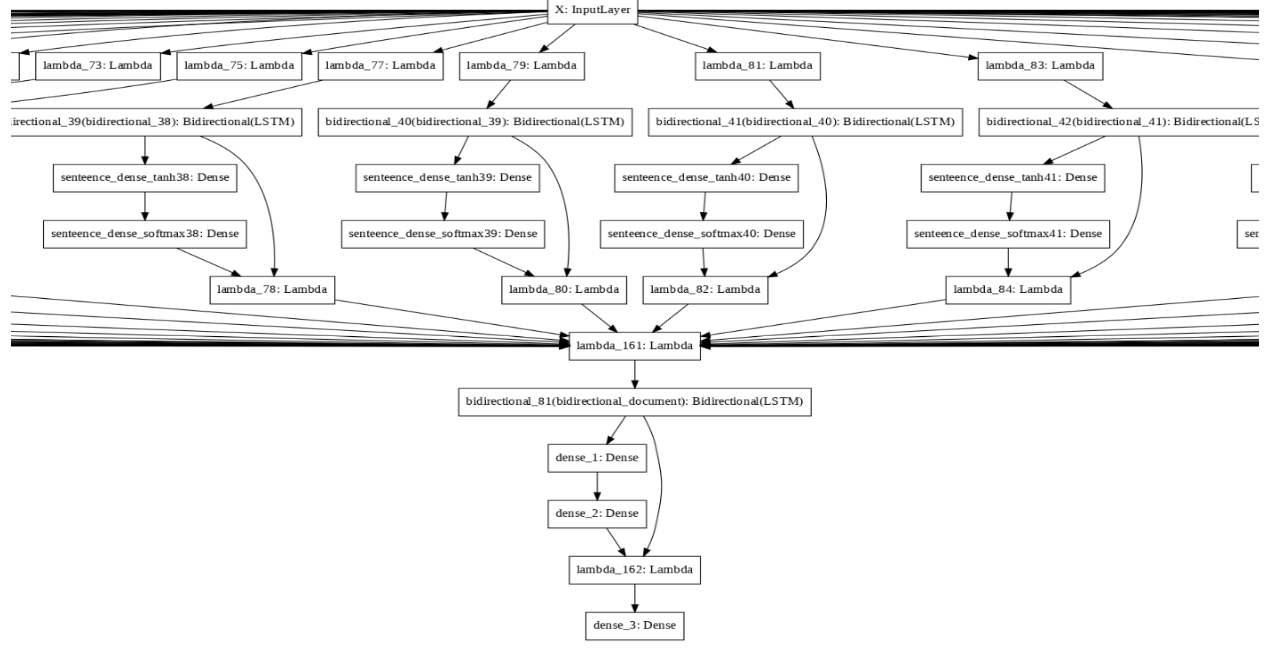
\includegraphics[scale=0.7]{Model.PNG}
    \caption{Our Model }
    \label{fig:model}
\end{figure}

\subsection{Model Architecture}
The model (figure \ref{fig:architecture}) is built from 3 levels hierarchy. It receives as an input a multidimensional matrix representing a document. The matrix built from list of sentences, each one of them is a list of words embeddings.

The first level in the model's hierarchy is built from multiple blocks of LSTM + Attention, each one of them receives a sentence as input (word after word), and the output of the block is a vector representing "sentence embeddings".

The second level in the model's hierarchy is a single block of LSTM + Attention that receives all the sentences embeddings (sentence after sentence), and the output of the block is a vector representing "document embeddings".

The last level in the model's hierarchy is a custom layer that receives as an input the document embeddings, all the sentences embeddings and the return sequence of the LSTM from the second level. This layer makes classification by extracting features that decides the probability of each sentence to be in the summary.

\begin{figure}
\begin{minipage}{.5\textwidth}
    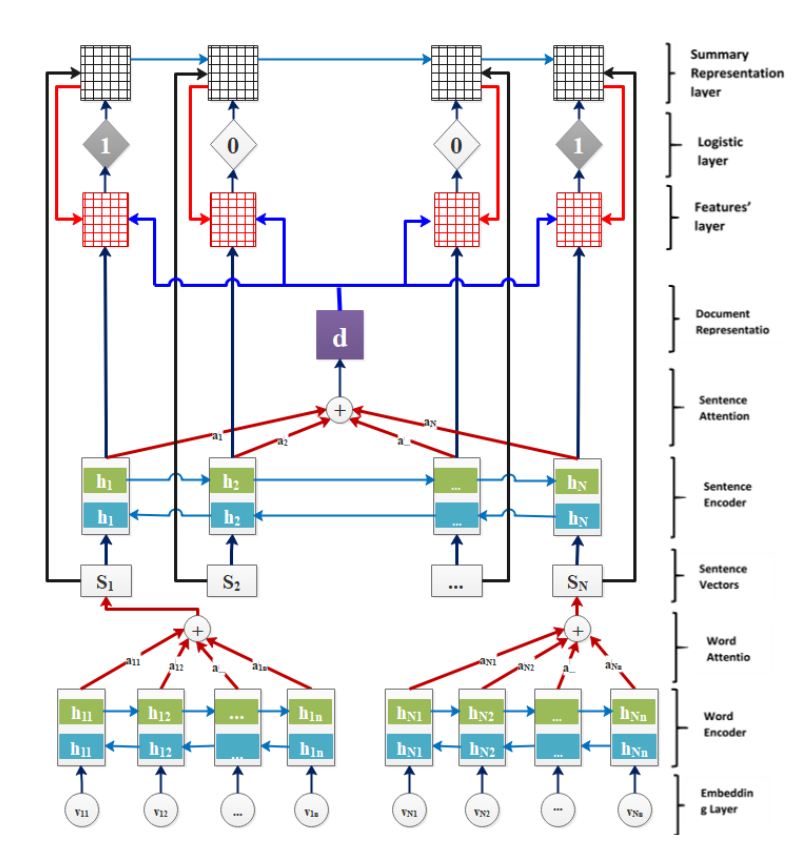
\includegraphics[scale=0.7]{Architecture.PNG}
    \caption{The Model's Architecture}
    \label{fig:architecture}
\end{minipage}
\begin{minipage}{.5\textwidth}
    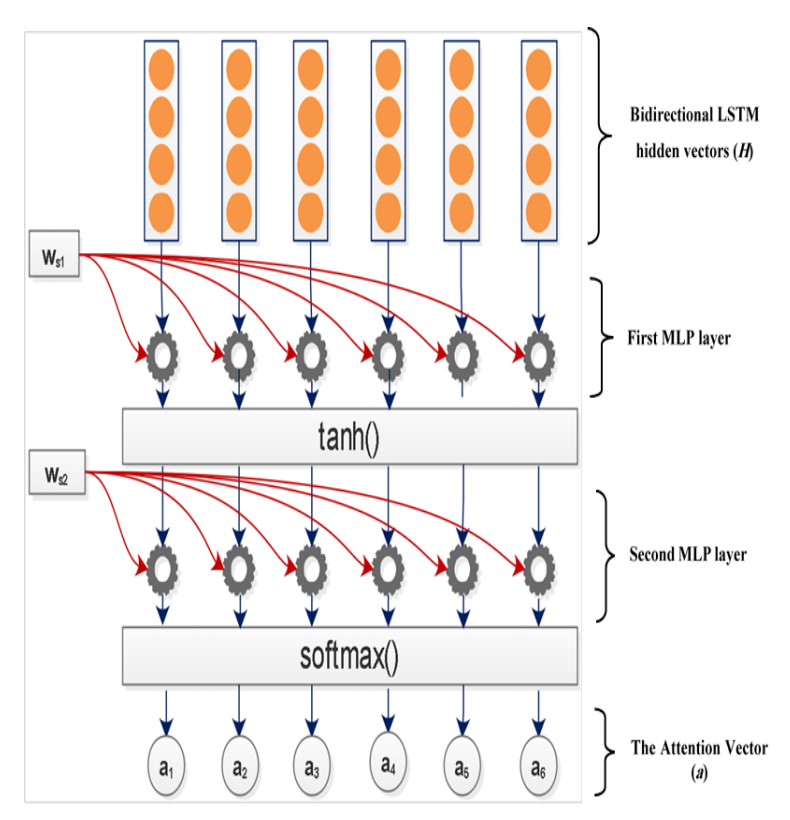
\includegraphics[scale=0.7]{Attention.PNG}
    \caption{The Attention Layer}
    \label{fig:attention}
\end{minipage}
\end{figure}

\subsection{Attention Layer}
The attention layer (figure \ref{fig:attention})  receives as an input the results of each timestamp in the LSTM, and passes into 2 dense layers:
\begin{enumerate}
    \item tanh - for non-linearity
    \item softmax - to get probabilities
\end{enumerate}

Then, the output probabilities are multiplied by the input embeddings, and then all the results are summed into one vector.

\subsection{Classification Layer}
In the classification layer we extracted features and used them to calculate the sentences' probabilities. The features are:
\begin{itemize}
    \item Information content - represented as sentence's embeddings
    \item Salience - represented as multiplication of sentence's embeddings and the document's embeddings
    \item Novelty - represented as multiplication of sentence's embeddings and another parameter called "The document's state". This parameter is the sum of probabilities of the sentences before the current. The probability decreases when the current sentence is more advanced in the document.
    \item Position - the result of the final LSTM at the timestamp of the sentence
\end{itemize}
All these features are learnable. The full description of how to calculate each one of them is written in the article.

\subsection{Data Preparation}
We used CNN/Daily-Mail dataset. After a long search we found an article (\href{https://arxiv.org/pdf/1611.04230.pdf}{R. Nallapati, F. Zhai, and B. Zhou, ‘‘SummaRuNNer: A recurrent neural network based sequence model for extractive summarization of documents’’}) that implemented the data preparation to a convenient structure. We used this data as a starting point, then we still had to separate the sentences and their labels, tokenize the sentences, calculate word embeddings and create input matrix with the structure that fits our model:
\begin{itemize}
    \item N samples
    \item 80 sentences per sample
    \item 50 words per sentence
    \item Vector of size 300 as word embeddings
\end{itemize}

\section{Challenges}
During the work we encountered many challenges, both in understanding some thins and also in the implementation itself. In the end we found the ways to deal with most of them. Here are some of the main challenges.
\begin{itemize}
    \item We couldn't use the sequential api - so we had to create more basic items (layers) and connect them manually using Keras functional api.
    \item We learned how to create shared layers outside the model and connect them to the model. These layers are the blocks that handle the words and create the sentence embeddings. The reason these layers are initiated outside the main model and are called from inside the model is because their weights are shared between all samples.
    \item We learned how to create custom layer with Keras (the classification layer). During the implementation of the layer we found some mistakes in the article's notations and mismatch in sizes of the features. We tried to reach the article's authors but they didn't answer. Because of this, we trained the final model twice - first with the classification layer using the correct size of the features (as we understood it should be) and second with a dense softmax layer instead of this custom layer.
    \item Because we had to make a classification to each sentence - we couldn't use the regular cross-entropy loss function of Keras, and we had to implement our own loss function.
    \item We faced memory issues in Google Colab so we had to explore and try many parameters to optimize the memory usage while not harming the model. Therefore, we preferred to decrease the size of each sample instead of using less samples. In each sample we reduced the word embeddings size, and the number of sentences per document. We tried to reduce the maximal number of words in each sentence but it did harm the model (because sometimes the last words in the sentence makes it important). By changing number of sentences we basically changed the problem at hand.
\end{itemize}

\section{Experimental results}
The proposed method to measure the model in the article is ROUGE (Recall-Oriented Understudy for Gisting Evaluation). 
ROUGE compares n-grams between the model's summary and the given input summary. The article's authors measured their model with ROUGE-1, ROUGE-2 and ROUGE-L (Longest Common Subsequence). The reason they chose ROUGE method is because they compared their model to other models that are not extractive and therefore doesn't have labels for sentences. They also explain that ROUGE is not necessarily good because it doesn't indicate on readability of the summary.

We didn't implement the ROUGE measurement on our model because we didn't have to compare our results to other abstractive models - we used the labels and tested our model on the test data.

As a result of memory problems with free Google Colab we had to run the model compromising some parameters. Be it the number of examples, the number of sentences per document, or the size of each word embedding. Eventually we chose 4 different configurations as described in the table below. Those configurations maxed some parameters (embedding size, number of examples) and still managed to fit in memory and not crash. As one can see the results did not exceed the 11\% accuracy mark. We hope that with better machine to run the model those compromises can be mitigated to achieve better results.

\begin{center}
\begin{tabular}{ |c|c|c|c|c| } 
 \hline
\diagbox{Param}{Conf \#} & 1 & 2 & 3 & 4 \\\hline
Sentences per doc & 40 & 10 & 40 & 10 \\\hline
 Words per sentence & 30 & 40 & 30 & 40 \\\hline
 Words embeddings size & 50 & 300 & 50 & 300 \\\hline
 \# of samples & 10,000 & 20,000 & 10,000 & 20,000 \\\hline
 Classification layer & custom & custom & dense & dense \\\hline
 Accuracy & 6\% & 10\% & 5\% & 11\% \\\hline
 Results & 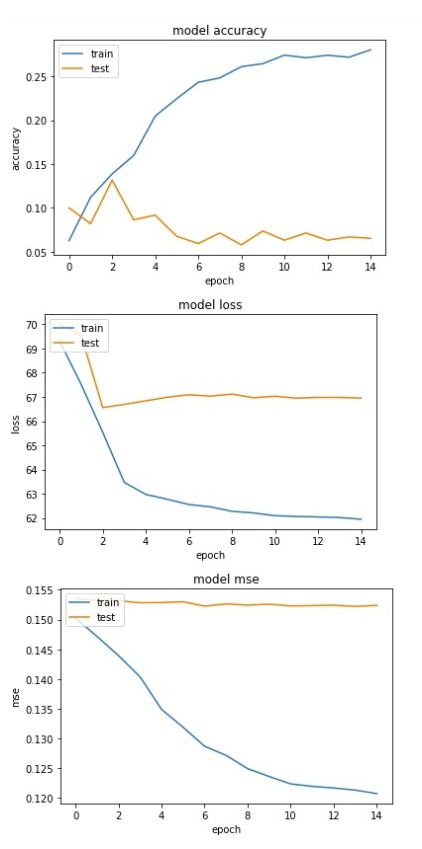
\includegraphics[width=0.2\textwidth]{images/Conf_1.PNG} & 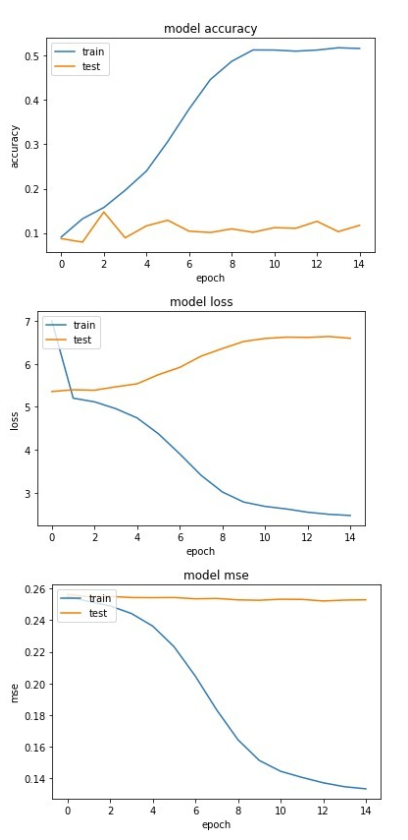
\includegraphics[width=0.2\textwidth]{images/Conf_2.PNG} &  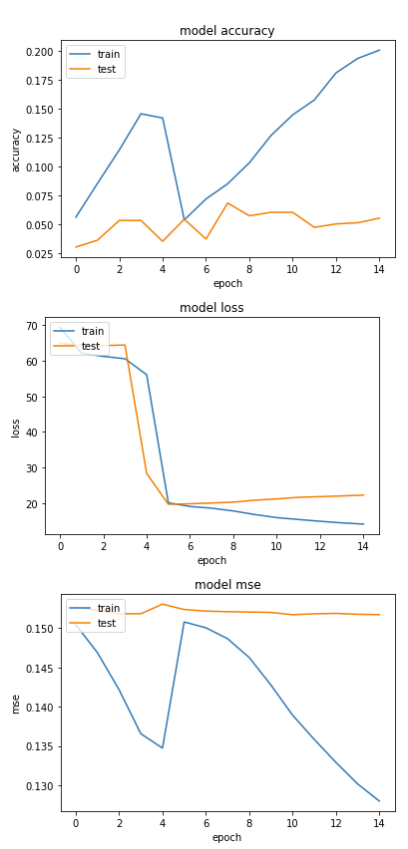
\includegraphics[width=0.2\textwidth]{images/Conf_3.PNG} & 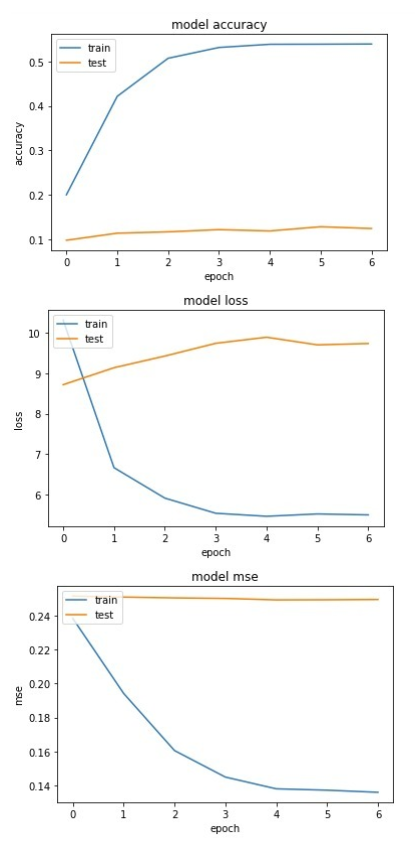
\includegraphics[width=0.2\textwidth]{images/Conf_4.PNG} \\\hline
\end{tabular}
\end{center}

Results Conclusions:
\begin{itemize}
    \item The architecture with the custom layer over-fitted to train from the 4th epoch. It could continue working more but Colab disconnected so we managed to run it 15 epochs.
    \item The architecture with the dense arrived to early stopping after 6 epochs only, meaning that there was a limit to the over-fit that it could made to the train (make sense, less parameters).
    \item In every configuration we couldn't reach more then 11\% accuracy on the test and validation.
    \item We could use different probability threshold for classification of 1, and maybe get better results. It could be an idea for future research. We tried it manually and it looked promising but we did not automate it.
\end{itemize}

\section{Discussion}
The project was very interesting and challenging. For both of us it was the first time we implemented an article from A to Z completely by ourselves. During the work we faced much more challenges and difficulties then we thought we would, and it made us read and explore more about neural networks in general and especially about implementation details with Keras. In the end of it, we both feel proud that we succeeded to overcome the obstacles and build a working model.

As a future work we think it might be interesting to build some abstractive summarization model and connect it to our model, with lower probability threshold for classification of 1. So basically our model will perform as a filter of the non relevant sentences and shorten the document, and the abstractive model would  generate a summarization based on that.

In conclusion, we enjoyed working on the project, it was a great opportunity to learn about building complex neural networks for a real-life NLP problem and we made the most of it.

\section{Code}
The code is \href{https://colab.research.google.com/drive/1fc2GYdHcewXZRS-pU1ZDqntKKjulvFlx}{here: https://colab.research.google.com/drive/1fc2GYdHcewXZRS-pU1ZDqntKKjulvFlx}.
\bibliographystyle{plain}
\bibliography{references}
\end{document}
